\chapter{Konsep Dasar Algoritma dan Pemrograman}\label{ch:konsepDasarAlgoritma}

\section{Struktur Dasar Algoritma}

\newthought{Pada bab sebelumnya, kita mempelajari bahwa program merupakan kumpulan dari algoritma-algoritma}. Algoritma sendiri di dalamnya juga merupakan kumpulan dari struktur-struktur dasar pembangun algoritma. Terdapat tiga jenis utama struktur algoritma yaitu : 

\begin{enumerate}
	\item \textbf{\textit{Sequence} (Runtunan)}, merupakan struktur algoritma paling dasar yang berisi rangkaian instruksi/pernyataan(\textit{statement}) yang diproses secara sekuensial, satu per satu, mulai dari instruksi pertama sampai instruksi terakhir. Salah satu contoh \textit{Sequence} ada pada contoh bab sebelumnya yaitu algoritma memindahkan isi dari kedua gelas (Gambar \ref{fig:illustrasiSequence}). 
	\begin{figure}
		\centering
		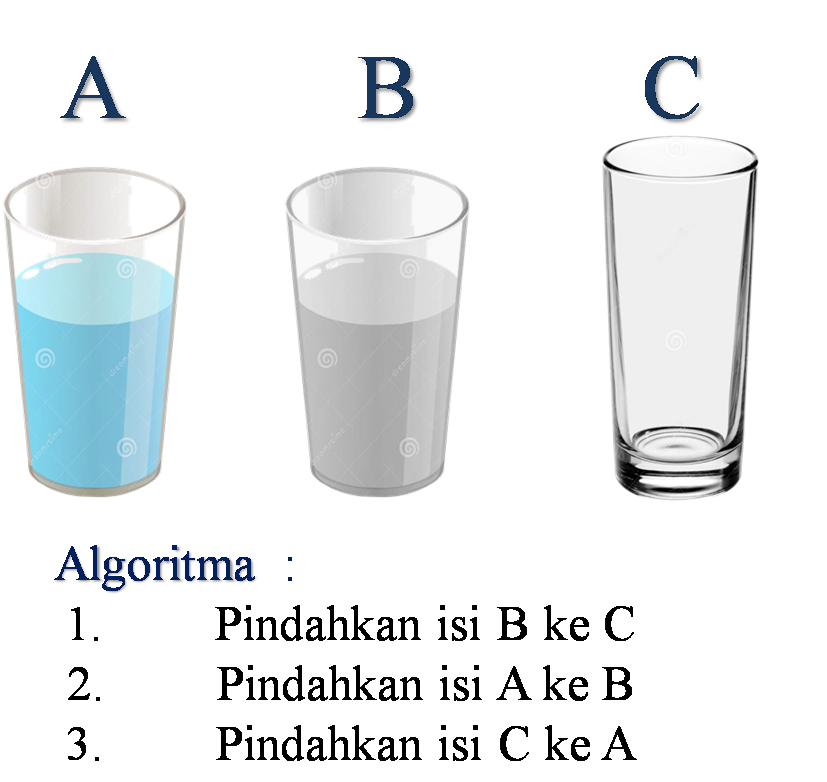
\includegraphics[scale=0.4]{fig/1/Gambar13.png}	
		\caption{Illustrasi \textit{sequence}. Ada 3 \textit{statement} di dalam  1 \textit{sequence}untuk memindahkan isi dari kedua gelas.}
		\label{fig:illustrasiSequence}
	\end{figure}
	\FloatBarrier
	\item \textbf{\textit{Selection/Branching} (Pemilihan / Percabangan)},) merupakan struktur algoritma yang akan digunakan dimana jika terdapat alternatif/pilihan beberapa pernyataan yang akan dijalankan jika memenuhi syarat tertentu. Percabangan dapat diibaratkan sebagai persimpangan jalan yang harus dipilih, jika kita memilih sebuah jalan dari persimpangan tersebut sudah pasti kita tidak akan menjalani yang lainnya. Salah satu contoh percabangan dapat dilihat pada contoh ``Algoritma Memilih Tempat Pembuangan'' (Gambar \ref{fig:illustrasiBranching}).
		\begin{figure}
			\centering
			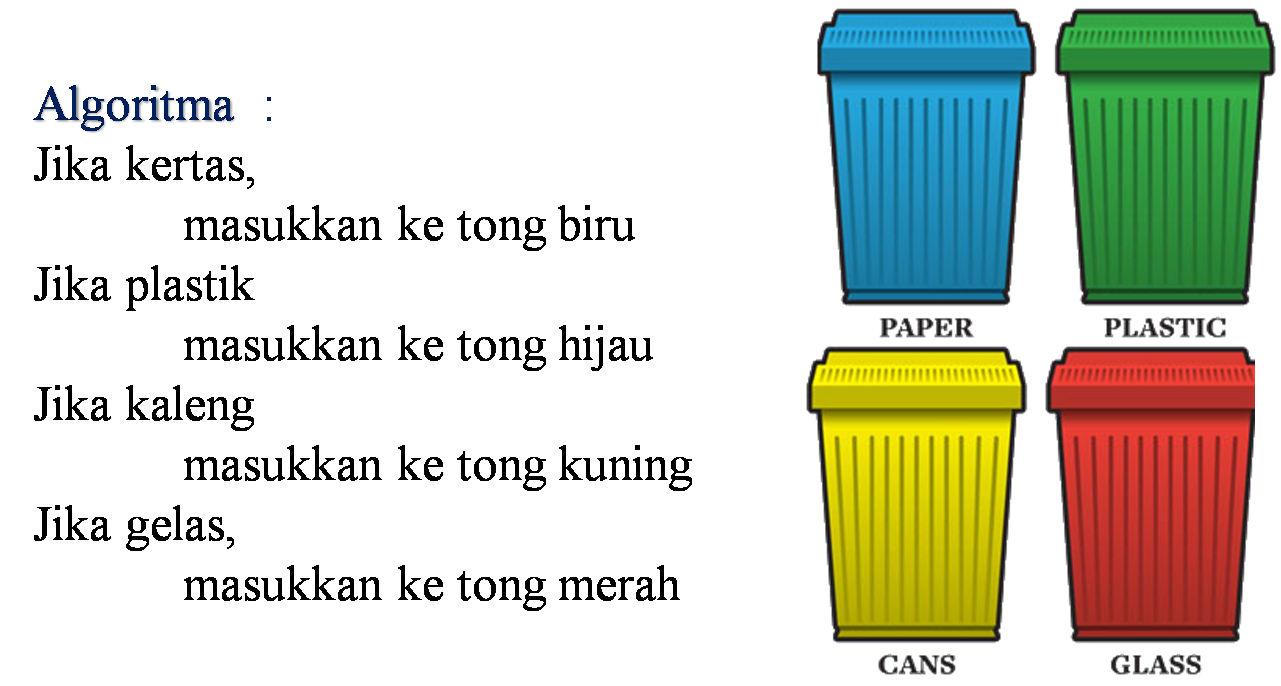
\includegraphics[scale=0.4]{fig/1/Gambar14.png}	
			\caption{Illustrasi \textit{Selection/Branching}. Di sini salah satu dari keempat tong harus dipilih ketika membuang sampah.}
		\label{fig:illustrasiBranching}
		\end{figure}
	\FloatBarrier
	\item \textbf{\textit{Repetition/Looping} (Pengulangan)}, merupakan struktur algoritma yang akan digunakan dimana jika terdapat pengulangan terhadap satu pernyataan tertentu. Beberapa contoh nyata penggunaan pengulangan misalnya pada saat harus melakukan penelusuran angka-angka voucher dari awal sampai akhir. Contoh lain yang lebih dekat dengan dunia nyata misalnya adalah algoritma ``pembagian permen'' (Gambar \ref{fig:illustrasiLoop}).
		\begin{figure}
		\centering
		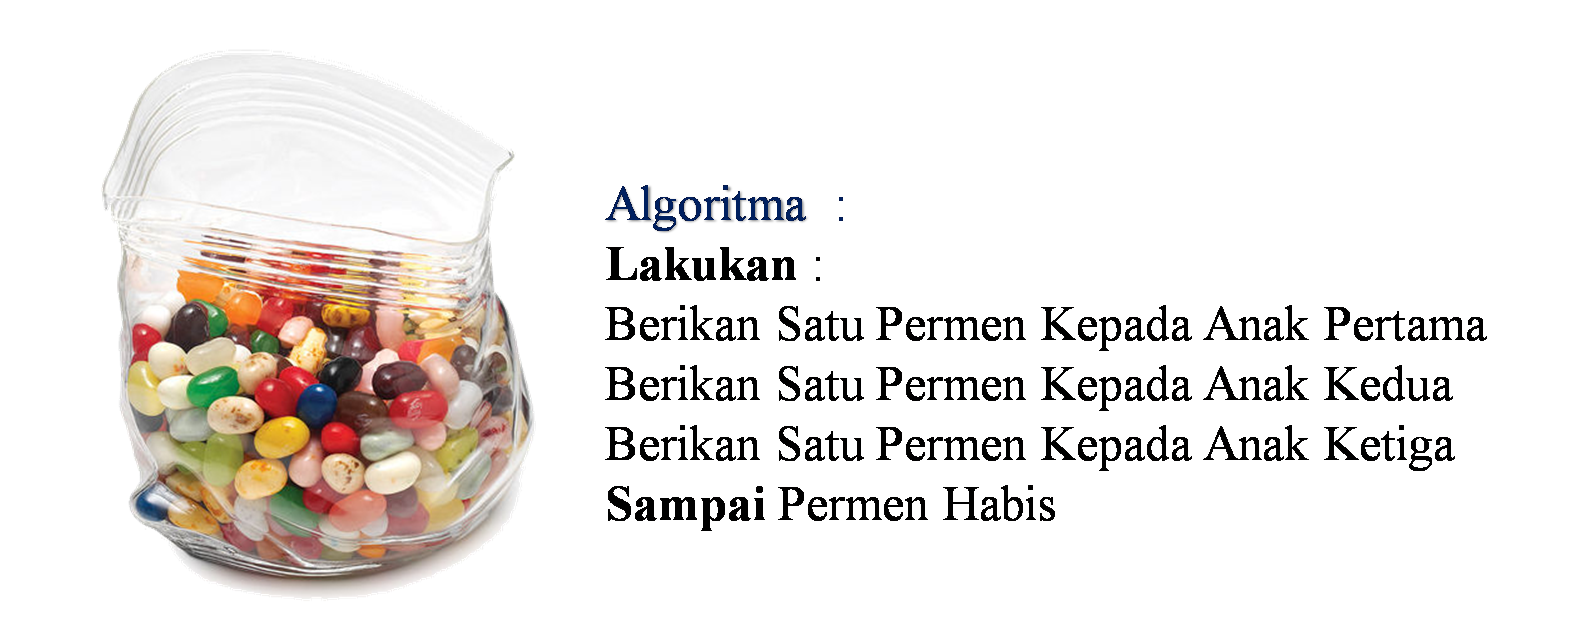
\includegraphics[scale=0.4]{fig/1/Gambar15.png}	
		\label{fig:illustrasiLoop}
		\caption{Illustrasi \textit{Repetition/Looping}. Di sini pemberian permen kepada ketiga anak harus dilakukan terus menerus sampai jumlah permen habis.}
		\end{figure}
\end{enumerate}

Percabangan dan Perulangan akan dibahas lebih lanjut pada pertemuan selanjutnya. Perlu diperhatikan bahwa masing-masing dari struktur dasar ini tidak berdiri sendiri dan terpisah. Pada kasus pembuatan algoritma sebenarnya, struktur dasar ini akan saling dipasangkan satu sama lain. Beberapa kasus dari penggabungan struktur dasar ini adalah sebagai berikut : 
\begin{itemize}
	\item Perulangan bersarang
	\item	Percabangan bersarang
	\item	Percabangan dalam Percabangan 
	\item	Perulangan dalam Percabangan 
	\item	Percabangan dalam Perulangan 
	\item	Perulangan dalam Percabangan
	\item	Perulangan dalam Perulangan dengan Percabangan
	\item	Berbagai kombinasi lainnya
\end{itemize}


%\subsection{Tipe Data}
\section{Tipe Data dan Variabel}
Dalam mengubah masalah sehari-hari menjadi algoritma, kemudian dari algoritma menjadi bahasa program, kita harus melakukan proses penyederhanaan informasi-informasi dari masalah tersebut. Misalnya, ada masalah menukar isi dalam gelas, kita memerlukan sesuatu yang dapat merepresentasikan/mewakili informasi isi dari gelas seperti sirup atau air  ke dalam algoritma atau bahasa program. Untuk penyelesaian, kita memiliki beberapa alternatif seperti apakah kita akan mewakilinya dengan kata atau dengan nilai. Dari sinilah muncul konsep tipe data dan variabel dalam algoritma. Pada pengenalan akan dikenalkan dahulu beberapa tipe data dasar, kemudian seiring dengan perkembangan mata kuliah, tipe data baru dan yang lebih muktahir akan diperkenalkan.

\subsection{Tipe Data}	
Beberapa tipe data dasar yang umum\footnote{Tipe data ini disebut juga sebagai tipe data primitif} adalah sebagai berikut: 
\begin{itemize}
	\item Bilangan Bulat: Integer, Long
	\item	Bilangan Riil: Float
	\item	Logika: Boolean
	\item	Karakter: Char
	\item	Kumpulan Karakter: String 
\end{itemize}

Secara umum, tipe data inilah yang digunakan untuk mewakili kasus-kasus dunia nyata yang akan diterjemahkan menjadi algoritma kemudian menjadi bahasa program. 

%\subsection{Variabel}
\subsection{Variabel}
VARIABEL pada algoritma digunakan untuk menampung nilai dengan tipe data tertentu. Variabel dimaksudkan untuk menyimpan informasi berupa nilai yang dapat secara dinamis berubah, diberi nilainya ataupun dibaca kembali pada saat dibutuhkan. Jika ``Sirup'' merupakan sebuah nilai dengan tipe data String, maka kita dapat menampungnya dalam sebuah variabel yang bernama $GelasA$. Setelah itu nanti $GelasA$ akan berubah nilainya ketika ditukar dengan isi dari $GelasB$ dan seterusnya.
\begin{contoh}
	\textbf{Penggunaan variabel}\\
	$a$ = 5 $\rightarrow$ Memasukkan nilai 5 ke variabel `$a$'.\\
	$b$ = 7 $\rightarrow$ Memasukkan nilai 7 ke variabel `$b$'.\\
	$a$ = $b$ $\rightarrow$ Memasukkan nilai variabel `$b$' ke variabel `$a$'. Kedua variabel sekarang bernilai 7.\\
	$a$ = $b$ = 9 $\rightarrow$ Memasukkan nilai 9 ke variabel `$a$' dan `$b$'.\\
\end{contoh}

Beberapa peraturan dalam penggunaan variabel adalah sebagai berikut: 
\begin{itemize}
	\item Penamaan variabel sebaiknya eksplisit sesuai dengan tujuan dari pembuatan variabel tersebut. Misalnya : $GelasA$ daripada $A$, $GelasB$ daripada $B$. Tetapi juga tidak usah terlalu panjang dan detil seperti misalnya $GelasAWarnaPutihdanBaru$. Cukup sampai bisa dipahami saja.
	\item	Penamaan variabel tidak boleh melibatkan spasi!  Misalnya : $Gelas\,A$ dan $Gelas\,B$ adalah salah, sedangkan $GelasA$ dan $Gelas\_B$ benar
	\item	Penamaan variabel sebaiknya dimulai dengan huruf. Misalnya : $123Panjang$ adalah salah. $Panjang123$ adalah benar. 
	\item	Pada bahasa pemrograman tertentu, penamaan variabel biasanya \textit{case-sensitive}. Misalnya : $nama$ berbeda dengan $Nama$ berbeda dengan $NAMA$ berbeda dengan $namA$.
	\item	Penamaan variabel jangan bertabrakan dengan \textit{reserved-word} pada bahasa pemrograman tertentu!
\end{itemize}

Beberapa hal yang akan sering kita lakukan pada pembuatan variabel di algoritma adalah deklarasi dan definisi. Proses inisialisasi awal variabel yang melibatkan pemberian tipe data disebut deklarasi. Proses pemberian nilai pada variabel disebut definisi.

\marginnote[-4cm]{
\begin{konsep}
Jika terdapat 4 variabel, yaitu: $a$, $b$, $c$, dan $d$ dengan nilai $a$ = 1, $b$ = 2, $c$ = 3, dan $d$ =  4. Tuliskan sebuah algoritma untuk menukarkan isi variabel tersebut sehingga nilainya menjadi $b$ = 1, $c$ = 2, $d$ = 3, dan $a$ = 4. Usahakan agar pertukarannya minimum.
\end{konsep}}

\subsection{Variabel dan Tipe Data Pada Python}
Khusus pada bahasa pemrograman Python, tidak ada deklarasi variabel yang dilibatkan \footnote{Bahasa pemrograman yang perlu deklarasi disebut \textit{statically typed programming language} contohnya: C++, Java, C\# dan sebagainya. Sedangkan yang tidak perlu deklarasi disebut \textit{dynamically type programming language} contohnya Python, Ruby, Javascript dan sebagainya}. Pembuatan variabel pada Python pada umumnya langsung dibuat melalui proses definisi. Setelah proses definisi, Python akan langsung menyesuaikan tipe data pada variabel tersebut. Lihat Gambar \ref{fig:definisiVar} untuk lebih jelas. 
	\begin{figure}
		\centering
		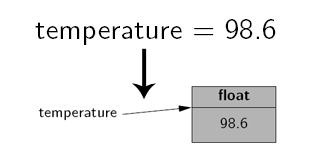
\includegraphics[scale=0.75]{fig/1/definisiVar.png}
		\caption{Definisi variabel di Python}
		\label{fig:definisiVar}
	\end{figure}

Perlu diingat juga, peraturan penggunaan variabel sama seperti sebelumnya \footnote{Untuk lebih jelas silakan dibaca di \url{http://legacy.python.org/dev/peps/pep-0008/\#naming-conventions}}. Dengan tambahan daftar \textit{reserved-words} ada di Gambar \ref{fig:reservedWords}.
		\begin{figure}
		\centering
		\includegraphics[scale=0.4]{fig/1/Gambar17.png}
		\caption{Daftar \textit{reserved-words} di Python. Nama variabel tidak boleh menggunakan nama di daftar ini}
		\label{fig:reservedWords}
		\end{figure}


%\subsection{Operator}
\section{Operator}
Pada algoritma, operator berfungsi untuk menghubungkan satu atau lebih variabel sehingga menghasilkan nilai baru. Beberapa operator dasar ditampilkan di Tabel \ref{tbl:operatorAritmatika}, \ref{tbl:operatorLogika}, dan \ref{tbl:operatorPerbandingan}.

\FloatBarrier
\begin{itemize}

	\item \textbf{Operator Aritmatika}
			\large
			\begin{table}
				\centering
				\begin{tabular}[h!]{| c | c | c |}
				\hline	
				\textit{Operasi} & \textit{Simbol} & \textit{Python} \\ \hline
				Penambahan & + & + \\ \hline
				Pengurangan & - & - \\ \hline
				Perkalian & x & * \\ \hline
				Pembagian & / & / dan // \\ \hline
				Perpangkatan & \^{}  & ** \\ \hline
				Hasil Sisa Bagi & \% & \% \\
				\hline
				\end{tabular}
				\caption{Operator Aritmatika}
				\label{tbl:operatorAritmatika}
		\end{table}
	\FloatBarrier
	\item \textbf{Operator Logika}
			\large
			\begin{table}
				\centering
				\begin{tabular}[h!]{| c | c | c |}
				\hline	
				\textit{Operasi} & \textit{Simbol} & \textit{Python} \\ \hline
				Dan & $\&\&$ & AND \\ \hline
				Atau & $\|$ & OR \\ \hline
				Bukan & $!$ & NOT \\ 
				\hline
				\end{tabular}
				\caption{Operator Logika}
				\label{tbl:operatorLogika}
		\end{table}

\FloatBarrier	
	\item \textbf{Operator Perbandingan}
			\large
			\begin{table}
				\centering
				\begin{tabular}[h!]{| c | c | c |}
				\hline	
				\textit{Operasi} & \textit{Simbol} & \textit{Python} \\ \hline
				Sama Dengan & $=$ & == \\ \hline
				Tidak Sama Dengan & $\neq$ & != \\ \hline
				Lebih Besar & $\geq,>$ & $>=,>$ \\ \hline
				Lebih Kecil & $\leq,<$ & $<=,<$ \\
				\hline
				\end{tabular}
				\caption{Operator Perbandingan}
				\label{tbl:operatorPerbandingan}
		\end{table}
\end{itemize}

\FloatBarrier

Sama seperti pada matematika dimana pada sebuah perhitungan, operator kali akan dijalankan terlebih dahulu dibanding penambahan dan pengurangan karena memiliki kekuatan operator yang lebih tinggi. 
	\begin{figure}
	\includegraphics[scale=0.50]{fig/1/Gambar21.png}
	\caption{Operator Precedence}
	\label{fig:operatorPrecedence}
	\end{figure}	
Anda boleh mengabaikan operator-operator yang belum diketahui diatas, cukup mengetahui urutan kekuatan operator-operator dasar terlebih dahulu.	

\section{Mendefinisikan Permasalahan}

Untuk setiap permasalahan komputasional, ada cara untuk mendefinisikannya. Definisi dibutuhkan untuk menyelesaikan permasalahan tersebut. Definisi dari sebuah permasalahan komputasional bisa dari sangat sederhana seperti di Contoh \ref{cth:pengurutan} sampai ke definisi yang sangat kompleks seperti contohnya permasalahan identifikasi DNA manusia di \textit{Human Genome Project} yang memerlukan algoritma yang sangat kompleks.

Sampai bab ini, kita sudah memiliki pengetahuan yang cukup untuk membuat salah struktur algoritma dasar yaitu \textit{sequence}. Kembali lagi perlu diingatkan bahwa algoritma dibuat untuk menyelesaikan masalah. Ketika bertemu masalah, agar cara berpikir kita rapi dan efektif, maka alangkah baiknya mengikuti ``rule of thumb'' berikut ini: 
\begin{enumerate}
	\item Apa masukkan dari masalah ini ? Ini berhubungan dengan bentuk awal dari  masalah. Pertanyaan-pertanyaan ini selanjutnya boleh diperluas dengan memikirkan, berapa variabel yang dibutuhkan di awal? tipe variabel apa saja yang dibutuhkan  di awal ?
	\item Apa keluaran dari masalah ini ? Kapan algoritma akan berhenti ? Apakah algoritma cukup berhenti jika semua proses sudah dijalankan ?  Jika sudah berhenti variabel apa yang akan saya tampilkan kepada pengguna ? Atau bentuk output apa yang akan saya tampilkan kepada pengguna ?  Apakah 
	\item Terakhir, apa proses(algoritma inti) dari masalah ini ? Apakah saya cukup menggunakan runtunan ? Apakah perlu struktur dasar lainnya (Pertemuan berikut !) ? Operator-operator apa saja yang perlu saya gunakan. Perlukah ada variabel-variabel pembantu lainnya ?
\end{enumerate}
Berikut adalah definisi dari permasalahan pengurutan.
\begin{contoh}
\label{cth:pengurutan}
\textbf{Permasalahan Pengurutan (\textit{Sorting Problem})}\\
Diberikan sebuah rangkaian angka $A$, urutkan angka tersebut secara menaik (\textit{ascending}).\\
\textbf{Masukan:}\\
Sebuah rangkaian \textit{n} angka $\left\langle a_{1},a_{2},\ldots,a_{n} \right\rangle$.\\
Misalnya $A = \left\langle 31,41,59,26,41,58 \right\rangle$

\textbf{Keluaran:}\\ 
Permutasi dari \textit{array} angka A $\left\langle a_{1},a_{2},\ldots,a_{n}\right\rangle$ dengan kondisi $\acute{a_{1}} \leq\ \acute{a_{2}} \leq \acute{a_{3}} \ldots \leq \acute{a_{n}}$ \\
Misalnya $A = \left\langle 26,31,41,41,58,59 \right\rangle$
\end{contoh}
Berikut adalah definisi dari permasalahan Pencarian Bilangan Prima.
\begin{contoh}
\label{cth:prima}
\textbf{Permasalahan Pencarian Bilangan Prima}\\
Hasilkan serangkaian bilangan prima dari bilangan $2$ sampai dengan bilangan $n$.\\  
\textbf{Masukan:}\\
Sebuah bilangan bulat \textit{n} yang merupakan batas atas dari \textit{array} bilangan prima yang akan dihasilkan.\\
Misalnya $n = 10$\\
\textbf{Keluaran:}\\
Satu set (himpunan elemen yang tidak memiliki duplikat) bilangan $A$ yang terdiri dari bilangan $2$ sampai bilangan $n$ dimana setiap bilangan hanya memiliki dua pembagi saja yaitu $1$ dan bilangan itu sendiri.\\
Misalnya $A = \left\langle 2,3,5,7 \right\rangle$\\
\end{contoh}
Berikut adalah definisi dari permasalahan Penyebrangan Jembatan.
\begin{contoh}
\textbf{Permasalahan Penyebrangan Jembatan}\\
Ada empat orang yang berusaha menyebrangi sebuah jembatan di malam hari. Karena gelap, mereka membutuhkan sebuah obor untuk menyebrangi jembatan tersebut. Masalahnya adalah obor hanya ada satu dan jembatan tersebut hanya bisa disebrangi oleh dua orang dalam satu waktu yang bersamaan. Setiap orang memiliki waktu yang berbeda ketika menyebrangi jembatan tersebut. Orang pertama memakan waktu 1 menit, orang kedua 2 menit, orang ketiga 5 menit, dan orang keempat 10 menit. 
Agar semua orang bisa menyebrangi jembatan tersebut, maka obor harus dibawa pulang balik ketika melakukan penyebrangan. Hitunglah waktu paling minimal yang diperlukan untuk menyebrangi jembatan tersebut.\\
\textbf{Masukan:}\\
Empat buah bilangan $a,b,c,$ dan $d$ yang masing-masing merepresentasikan waktu yang diperlukan untuk menyebrangi jembatan tersebut untuk setiap orang.\\
Misalnya $a = 1, b = 2, c = 5, d = 10$\\
\textbf{Keluaran:}\\
Sebuah bilangan $z$ dimana bilangan tersebut merupakan waktu minimal yang diperlukan agar keempat orang tersebut berhasil menyebrangi jembatan tersebut.\\
Misalnya $z = 17$\\
\end{contoh}

\subsection{Pseudocode sebagai Notasi Algoritma}
Untuk setiap soal dari contoh-contoh sebelumnya bisa tersedia berbagai macam algoritma yang berbeda untuk menyelesaikannya. Salah satu contoh sederhana dari Contoh \ref{cth:pengurutan} adalah Algoritma \ref{algo:bubble} yang disebut juga dengan nama \textit{Bubble Sort}. 

Algoritma \ref{algo:bubble} ditulis dengan menggunakan pseudocode\sidenote{Pseudocode merupakan sebuah \textit{tool} untuk menuliskan algoritma. Pseudocode bukan merupakan bahasa pemrograman dan tidak bisa dieksekusi.}. Tujuan penggunaan pseudocode adalah agar tidak terikat terhadap bahasa pemrograman tertentu dan bisa lebih fokus ke algoritma saja. Akan tetapi, di mata kuliah ini, yang Pseudocode tidak digunakan melainkan langsung menggunakan Python.

\begin{algorithm}
	\caption{BUBBLE-SORT($A$)}
	\label{algo:bubble}
	\begin{algorithmic}[1]
	\FOR {$i = 1$ \TO $A.length-1$}
		\FOR {$j = i+1$ \TO $A.length$}
			\IF {$A[i] \leq A[j]$}
			\STATE $temp = A[i]$
			\STATE $A[i] = A[j]$
			\STATE $A[j] = temp$
			\ENDIF
		\ENDFOR
	\ENDFOR
	\end{algorithmic}
\end{algorithm}

\marginnote[-4cm]{\begin{konsep}
Berikan beberapa contoh definisi permasalahan komputasional (yang sederhana) yang anda ketahui lengkap dengan masukan dan keluaran dari permasalahan tersebut (min: 3 permasalahan)!
\end{konsep}}

\begin{konsep}
Asumsikan sebuah algoritma menyelesaikan sebuah permasalahan X yang memerlukan $f(n)$ mikrosekon. Untuk setiap $f(n)$ dan waktu $t$ di tabel berikut, tentukan nilai $n$ tertinggi yang bisa diselesaikan dalam waktu $t$.
\begin{figure}%
\centering
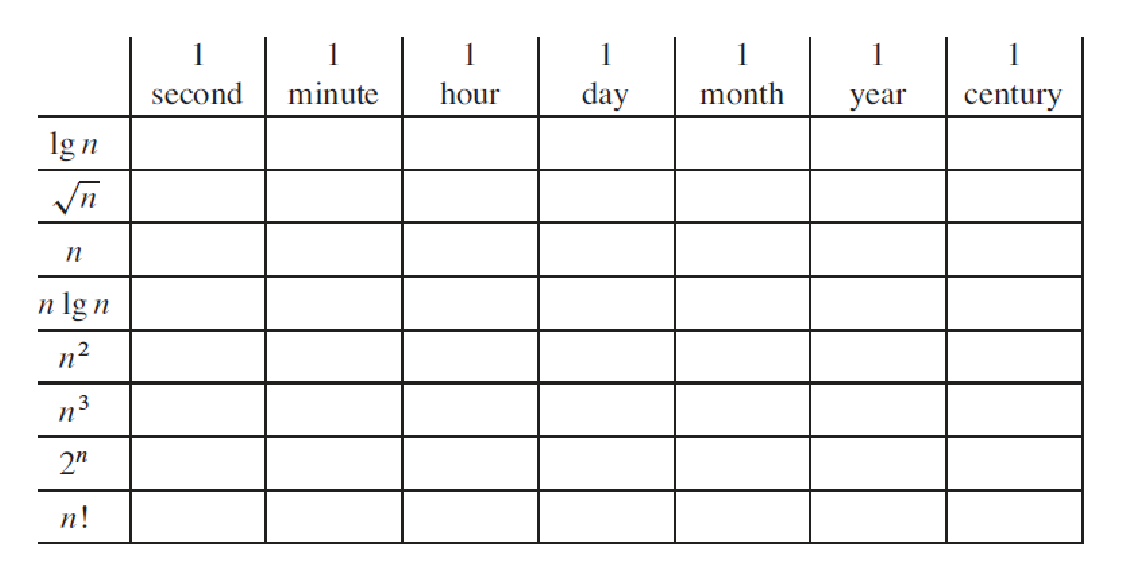
\includegraphics[scale=0.5]{fig/tableEksekusi.eps}%
\end{figure}
\end{konsep}
\newpage
\subsection{Flow Chart sebagai Notasi Algoritma}
Selain dengan menggunakan pseudocode, bisa juga menggunakan \textit{flow chart} untuk memvisualisasikan sebuah algoritma. Bentuk dari \textit{flow chart} untuk algoritma \ref{algo:bubble} bisa dilihat di gambar \ref{fig:flowchart}.

\begin{marginfigure}%
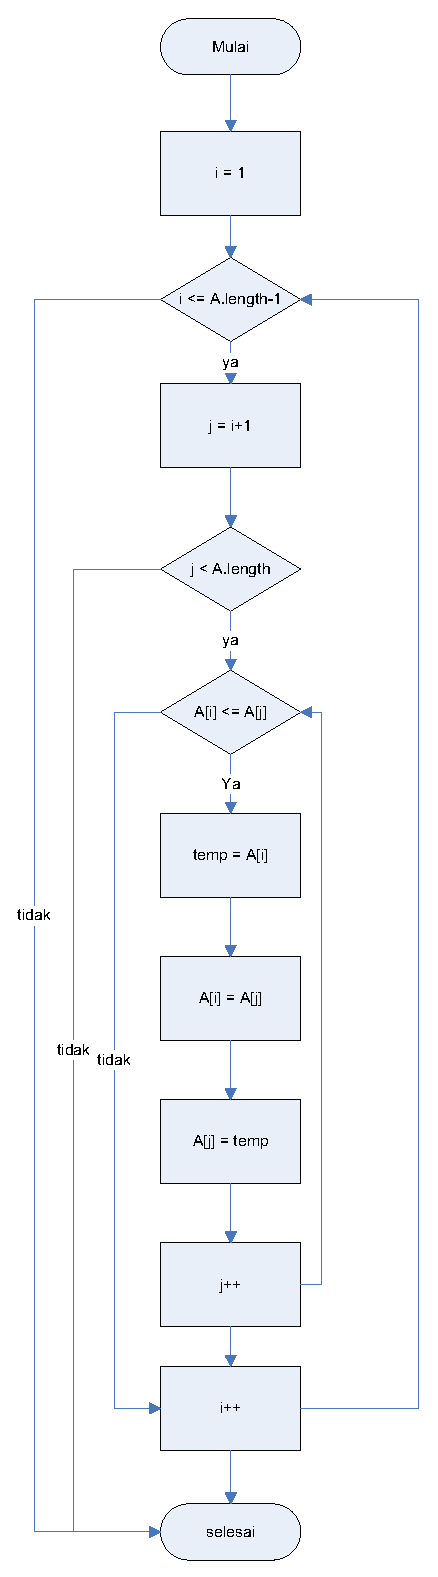
\includegraphics[scale=0.6]{fig/flowchart.eps}%
\caption{Flow Chart Bubble Sort}%
\label{fig:flowchart}%
\end{marginfigure}

\section{Implementasi algoritma ke bahasa pemrograman}
Algoritma \ref{algo:bubble} tidak bisa dijalankan secara langsung tanpa diimplementasi terlebih dahulu ke bahasa pemrograman. Bahasa yang digunakan di Algoritma \ref{algo:bubble} disebut sebagai \textit{pseudocode}. \textit{Pseudocode} sendiri tidak memiliki sebuah standar dalam penulisannya (tidak seperti bahasa Python yang memiliki aturan penulisan/sintaks). Penggunaan \textit{pseudocode} bisa berbeda-beda tergantung pada pembuat/penulisnya. 

Contoh implementasi Algoritma \ref{algo:bubble} ke bahasa pemrograman (Python) bisa dilihat di Listing \ref{lst:bubbleSortSimple}. Perlu diketahui, terdapat beberapa perbedaan mendasar antara algoritma dan listing program (misalnya indeks di algoritma dimulai dari 1 sedangkan di bahasa Python dimulai dari 0). 

\begin{listprog}{bubbleSort.py}
	\label{lst:bubbleSortSimple}
	\begin{lstlisting}[language=Python]
		A = [4,1,3,5,6,7,2]
		for i in range(1,len(A)):
				for j in range(i+1):
						if A[i]<=A[j]:
								temp = A[i]
								A[i] = A[j]
								A[j] = temp
		print A
	\end{lstlisting}
\end{listprog}

\newpage
\section{Latihan : Pengenalan II}

\begin{pemrograman}
Buatlah sebuah algoritma dan program dengan spesifikasi sebagai berikut  : 
\begin{enumerate}
	\item Menampilkan tulisan ``Halo, Siapa nama Anda ? ``, 
	\item Pengguna dapat menginput Nama setelah tulisan diatas, 
	\item Menampilkan tulisan ``Halo, Siapa nama Dosen Anda ? ``, 
	\item Pengguna dapat menginput Nama Dosen setelah tulisan diatas, 
	\item menuliskan pesan ``Selamat Menikmati Pengantar Algoritma, NAMAANDA dengan Dosen Pengampu Bapak / Ibu Dosen NAMADOSEN``
\end{enumerate}
\end{pemrograman}

\begin{pemrograman}
Lakukan perumusan masalah, pembuatan algoritma \& program untuk kasus ``Menukarkan Isi Gelas`` jika variabel pada masing - masing gelas memiliki tipe data String !
\end{pemrograman}

\begin{pemrograman}
Lakukan perumusan masalah, pembuatan algoritma \& program untuk kasus ``Menghitung Luas Persegi Panjang, Segitiga dan Lingkaran`` !
\end{pemrograman}

\begin{pemrograman}
Lakukan perumusan masalah, pembuatan algoritma \& program untuk kasus ``Konversi Suhu dari Celcius ke Reaumur, Farenheit, dan Kelvin`` !
\end{pemrograman}

\begin{pemrograman}
Lakukan perumusan masalah, pembuatan algoritma \& program untuk kasus ``Perhitungan panjang sisi miring untuk Segitiga`` !
\end{pemrograman}

\begin{pemrograman}
Seekor semut menempuh perjalanan sejauh $x$ cm. Buat algoritma \& program untuk mengkonversi jarak $x$ dalam km-m-cm. Misal $x$ = 261341
maka semut menempuh 2 km, 613 m, 141 cm
\end{pemrograman}

\begin{pemrograman}
Buat algoritma \& program yang dapat menghitung selisih waktu dari dua informasi waktu yang berbeda dengan format HH:MM:SS:mmm
\end{pemrograman}



%\FloatBarrier
%\subsection{Array}
%Array\sidenote{Di bahasa pemrograman Python, implementasi dari Array disebut sebagai List.} merupakan kumpulan dari variabel. Satu array bisa menampung beberapa data. Gambar \ref{fig:illustrasiArray} menunjukkan illustrasi dari sebuah array yang berkapasitas $j$.
%\begin{center}
	%\begin{figure}[htbp]%
		%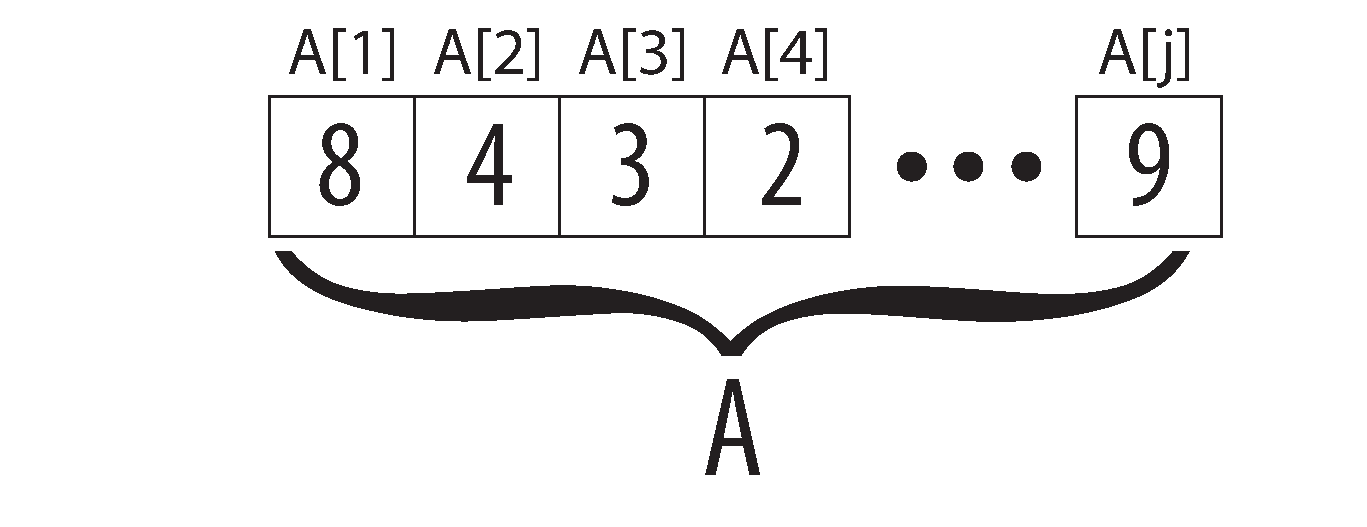
\includegraphics[scale=0.4]{fig/Array.eps}%
		%\caption{Illustrasi Array}%
		%\label{fig:illustrasiArray}%
	%\end{figure}
%\end{center}
%\begin{contoh}
	%\textbf{Penggunaan array}\\
	%$A[i] \rightarrow$ Mengakses lokasi ke $i$ dari array yang bernama $A$.\\
	%$A[4] \rightarrow$ Mengakses lokasi ke $4$ dari array yang bernama $A$.\\
	%$A[i..j] \rightarrow$ Menandakan kumpulan isi array $A$ yang terdiri dari elemen $A[1],\ A[2],\ A[3],\ \ldots,\ A[j]$.\\
	%$A[4] = 5 \rightarrow$ Memasukkan nilai 5 ke lokasi ke 4 dari array $A$.\\
	%$b = A[4] \rightarrow$ Memasukkan nilai lokasi ke 4 dari array $A$ ke variabel $b$. 
	%$A.length \rightarrow$ Menandakan besar/panjang dari array $A$.
%\end{contoh}

%\begin{pemrograman}
%Untuk melakukan latihan pemrograman algoritma dan Python di rumah, SPOJ merupakan website yang sangat berguna. SPOJ merupakan sebuah website \textit{Online Judge} dimana kita bisa melihat permasalahan-permasalahan yang menarik, menyelesaikan permasalahan tersebut dan meng-\textit{submit} solusinya ke SPOJ untuk di-\textit{judge}. SPOJ akan menentukan apakah solusi kita tepat atau salah. Diharapakan agar mahasiswa bisa menyelesaikan permasalahan SPOJ sebanyak mungkin untuk meningkatkan kemampuan pemrograman. Berikut langkah-langkah yang harus dilakukan di rumah.
%\begin{enumerate}
	%\item Buka website SPOJ (\url{www.spoj.pl})
	%\item Register di website SPOJ tersebut.
	%\item Baca tutorial di website SPOJ untuk memahami lebih lanjut di \url{http://www.spoj.pl/tutorials/}
	%\item Lihat daftar permasalahan (\textit{problems}) di website SPOJ di \url{http://www.spoj.pl/problems/classical}
	%\item Lihat permasalahan yang paling sederhana, yaitu permasalahan nomor 1 dengan CODE ``TEST'', atau dengan nama ``Life, the Universe, and Everything'' (\url{http://www.spoj.pl/problems/TEST/}).
	%\item Baca dan coba pahami soalnya.
	%\item Untuk percobaan akan dikasihkan solusinya sebagai berikut dalam bentuk \textit{source code} Python. 
	%\begin{listprog}{TEST.py}
	%\label{lst:TEST}
	%\begin{lstlisting}[language=Python]
		%k=input()
		%while k!=42:
			%print k
		%k=input()
	%\end{lstlisting}
	%\end{listprog}
	%\item Submit solusi tersebut di \url{http://www.spoj.pl/submit/}, pastikan pilihan \textbf{Language} adalah Python (python 2.7) dan Problem code adalah TEST.
	%\item Lihat hasilnya di \url{http://www.spoj.pl/status/} dan cari username anda di kolom USER. Jika ada tulisan ``accepted'' berarti anda telah berhasil menyelesaikan permasalahan tersebut. Jika tidak cek kembali apakah ada yang salah di langkah sebelumnya.
%\end{enumerate}
%\end{pemrograman}
